\documentclass{article}

\usepackage[utf8]{inputenc}
\usepackage[T1]{fontenc}
\usepackage[norsk,english]{babel}   %Norsk først så engelsk, så engelsk blir prioritert
\usepackage{graphicx}
\usepackage{amsmath}        %For å kunne skrive matte
\usepackage{listings}       %For å kunne skrive inn kode med fin formatering
\usepackage{multicol}       %Importerer pakken for multikolonner til teksten
\usepackage[margin=2.54cm]{geometry}    %Definerer hva bredden til teksten er
\usepackage{wrapfig}    %Importerer pakken for å ha bildene i teksten
\usepackage[font = small]{caption}

%Definerer hyperlinker og dens farger
\usepackage{hyperref}
\hypersetup{
    colorlinks,
    citecolor=blue,
    filecolor=black,
    linkcolor=blue,
    urlcolor=blue
}

%-----------------------------------

%Definerer farger til kodeeksemplene i PDF-en
\usepackage{color}

\definecolor{codegreen}{rgb}{0,0.6,0}
\definecolor{codegray}{rgb}{0.5,0.5,0.5}
\definecolor{codepurple}{rgb}{0.58,0,0.82}
\definecolor{backcolour}{rgb}{0.95,0.95,0.92}

\lstdefinestyle{mystyle}{
    backgroundcolor=\color{backcolour},
    commentstyle=\color{codegreen},
    keywordstyle=\color{magenta},
    numberstyle=\tiny\color{codegray},
    stringstyle=\color{codepurple},
    basicstyle=\footnotesize,
    breakatwhitespace=false,
    breaklines=true,
    captionpos=b,
    keepspaces=true,
    numbers=left,
    numbersep=5pt,
    showspaces=false,
    showstringspaces=false,
    showtabs=false,
    tabsize=2
}

\lstset{style=mystyle}

%------------------------------------

\setlength{\parindent}{0pt} %Ingen indent automaisk for nye linjer
%\setlength{\columnsep}{2mm} %Column separation - til multicolumn

%\setlength{\arrayrulewidth}{1mm}   %Hvilken tykkelse tabellene skal ha
\setlength{\tabcolsep}{2mm}     %Lengden mellom hver kolonne
\renewcommand{\arraystretch}{1.5}   %Hvor stor avstand det skal være mellom radene

\iffalse    %midlertidig endre bredden på teksten
If you want to change this temporarily, you can write:
\savegeometry{mydefaultgeometry}
\newgeometry{margin=3in}
And then later you can call:
\loadgeometry{mydefaultgeometry}
\fi

%for å fjerne overskriften "refrences" som kommer automatisk når man bruker bibtex
\usepackage{etoolbox}
\patchcmd{\thebibliography}{\section*{\refname}}{}{}{}

%----------------------------------------------------------------------------------------

\begin{document}

\addtocounter{page}{0}

\title{Project 4 \\
      \large For the course FYS3150}
\date{\today \\
    \vspace{1mm}
    \large Week 43 - ?}

\author{Erik Grammeltvedt, Erlend Tiberg North and Alexandra Jahr Kolstad}

\maketitle

%\newpage

%------------Her starter skrivingen-----------------------------------------

%\begin{multicols}{2}

\textbf{TING Å GJØRE}
\begin{itemize}
  \item a) ferdig
  \item b) alt
  \item c) alt
  \item d) alt
  \item e) alt
  \item f) alt
\end{itemize}


%-------------------- Abstract -------------------------------
\vspace{1cm}


\begin{center}

{\Large\textbf{Abstract}} \label{sec:Abstract}

\end{center}



\newpage

%------------------- Table of contents -----------------------

\vspace{1cm}

\tableofcontents

\vspace{1cm}

%-------------------- Introduction ------------------------------
\vspace{1cm}

\section{Introduction} \label{sec:Introduction}



%-------------------- Theory ------------------------------------
\vspace{1cm}

\section{Theory} \label{sec:Theory}

\subsection{Analytical solution for \texorpdfstring{ $2 \times 2$ }{text} lattice}

The energies in this lattice is given by the set $E_i = \{- 8 J, -4J, 0 , 4J, 8J \}$.

$$ \langle E \rangle = - 7.98393 $$
$$ \langle E^2 \rangle = 15.96786 $$
$$ C_V = (15.96 - (-7.98)^2) = -47.77528 \hspace{1cm} ???????? $$

$$ \langle M \rangle = 0 \hspace{1cm} ???????????????? $$
$$ \langle M^2 \rangle = 15.97322$$
$$ \chi = (15.97322 - (0)^2) = 15.97322 $$


\subsubsection{Partition function}

The partition function is given by the equation below.

\begin{equation} \label{eq:partitionfunction}
    Z = \sum_{i=1} ^{M} e^{- \beta E_i}
\end{equation} \\

The sum runs from 1 to $M$, which is 16 because of the $ 2 \times 2 $ lattice. To calculate the partition function we need to know that

\begin{equation*}
    2 \cosh (x) = e^x + e^{-x}
\end{equation*} \\

Calculating the partition function.

\begin{align*}
  Z &= \sum_{i=1} ^{M} e^{- \beta E_i} = \sum_{i=1} ^{16} e^{- \beta E_i} \\
  &= 1 \cdot e^{- \beta (-8J)} + 4 \cdot e^{- \beta (0J)} + 2 \cdot e^{- \beta (8J)} + 4 \cdot e^{- \beta (0J)}
  + 4 \cdot e^{- \beta (0J)} + 1 \cdot e^{- \beta (-8J)} \\
  &= e^{8 \beta J} + 4 + 2 \cdot e^{-8 \beta J} + 4 + 4 + e^{8 \beta J} \\
  &= 2 e^{8 \beta J } + 2 e^{-8 \beta J} + 12 \\
  &= 2 \left( e^{8 \beta J} + e^{- 8 \beta J} \right) + 12 \\
  &= 2 \left( 2 \cosh(8 \beta J) \right) + 12 \\
  &= 4 \cosh(8 \beta J) + 12
\end{align*} \\

The partition function for this system is therefore given by $Z = 4 \cosh(8 \beta J) + 12$.

\subsubsection{Energy and mean magnetization}

The expectation value of the energy is

\begin{equation}    \label{eq:expectationenergy}
    \langle E \rangle = \frac{1}{Z} \sum _{i=1} ^M E_i e^{- \beta E_i} \\
\end{equation} \\

In addition we need to know that

\begin{equation*}
    2 \sinh (x) = e^x - e^{-x}
\end{equation*} \\

The expectation value of the energy is

\begin{align*}
  \langle E \rangle &= \frac{1}{Z} \sum _{i=1} ^M E_i e^{- \beta E_i} \\
  &= \frac{1}{Z} \left[ 1 \cdot (-8J) e^{- \beta (-8J)} + 4 \cdot 0 + 2 \cdot (8J) e^{- \beta (8J)} + 4 \cdot 0 + 1 \cdot (-8J) e^{- \beta (-8J)} \right] \\
  &= \frac{1}{Z} \left[ - 8J e^{\beta 8J} + 2 \cdot 8J e^{- \beta 8J} - 8J e^{ \beta 8J} \right] \\
  &= \frac{2}{Z} \left[ - 8J e^{\beta 8 J} + 8 J e^{- \beta 8 J} \right] \\
  &= - \frac{16 J}{Z} \left( e^{8 \beta J} - e^{- 8 \beta J} \right) \\
  &= - \frac{16 J}{Z} (2 \sinh(8 \beta J) ) \\
  &= - \frac{32 J}{Z} \sinh(8 \beta J)
\end{align*} \\

The expectation value of the mean magnetization is

\begin{equation}    \label{eq:meanmagnetization}
    \langle M \rangle = \frac{1}{Z} \sum _{i=1} ^M M_i e^{- \beta E_i} \\
\end{equation} \\

For this system it is

\begin{align*}
  \langle M \rangle &= \frac{1}{Z} \sum _{i=1} ^M M_i e^{- \beta E_i} \\
  &= \frac{1}{Z} \left[1 \cdot 4 e^{- \beta (-8J)} + 4 \cdot 2 e^{- \beta (0J)} + 2 \cdot 0 + 4 \cdot 0 + 4 \cdot (-2) e^{- \beta (0J)} + 1 \cdot (-4) e^{- \beta (-8J)} \right] \\
  &= \frac{1}{Z} \left[ 4 e^{\beta 8J} + 8 - 8 - 4 e^{ \beta 8J} \right] \\
  &= \frac{1}{Z} \cdot 0 \\
  &= 0
\end{align*} \\


\subsubsection{Specific heat}

The specific heat is given by the equation

\begin{equation}    \label{eq:specificheat}
    C_V = \frac{1}{k_B T^2} \left( \langle E^2 \rangle - \langle E \rangle ^2 \right)
\end{equation} \\

Therefore the expectation value of the energy squared has to be calculated.

\begin{align*}
  \langle E^2 \rangle &= \frac{1}{Z} \sum _{i=1} ^M E_i^2 e^{- \beta E_i} \\
  &= \frac{1}{Z} \left[ 1 \cdot (-8J)^2 e^{- \beta (-8J)} + 4 \cdot 0 + 2 \cdot (8J)^2 e^{- \beta (8J)} + 4 \cdot 0 + 1 \cdot (-8J)^2 e^{- \beta (-8J)} \right] \\
  &= \frac{1}{Z} \left[ 64 J^2 e^{\beta 8J} + 2 \cdot 64 J^2 e^{- \beta 8J} + 64 J^2 e^{ \beta 8J} \right] \\
  &= \frac{2 \cdot 64 J^2}{Z} \left[ e^{\beta 8 J} + e^{- \beta 8 J} \right] \\
  &= \frac{128 J^2}{Z} (2 \cosh(8 \beta J) ) \\
  &= \frac{256 J^2}{Z} \cosh(8 \beta J)
\end{align*} \\

Now the specific heat can be calculated.

\begin{align*}
    C_V = \frac{1}{k_B T^2} \left( \langle E^2 \rangle - \langle E \rangle ^2 \right)
    &= \frac{1}{k_B T^2} \left( \frac{256 J^2}{Z} \cosh (8 \beta J) - \left( - \frac{32 J}{Z} \sinh(8 \beta J ) \right) ^2 \right)
\end{align*} \\


\subsubsection{Susceptibility}

The susceptibility is given by

\begin{equation}    \label{eq:susceptibility}
    \chi = \frac{1}{k_B T} \left( \langle M^2 \rangle - \langle M \rangle ^2 \right)
\end{equation} \\

The expectation value of the mean magnetization squared therefore has to be calculated.

\begin{align*}
  \langle M^2 \rangle &= \frac{1}{Z} \sum _{i=1} ^M M_i^2 e^{- \beta E_i} \\
  &= \frac{1}{Z} \left[1 \cdot 4^2 e^{- \beta (-8J)} + 4 \cdot 2^2 e^{- \beta (0J)} + 2 \cdot 0 + 4 \cdot 0 + 4 \cdot (-2)^2 e^{- \beta (0J)} + 1 \cdot (-4)^2 e^{- \beta (-8J)} \right] \\
  &= \frac{1}{Z} \left[ 16 e^{\beta 8J} + 16 + 16 + 16 e^{ \beta 8J} \right] \\
  &= \frac{1}{Z} \left[ 2 e^{8 \beta J} + 2 \right] \\
  &= \frac{32}{Z} \left( e^{8 \beta J} + 1 \right) \\
\end{align*}

Now calculating the susceptibility of the system.

\begin{align*}
    \chi &= \frac{1}{k_B T} \left( \langle M^2 \rangle - \langle M \rangle ^2 \right) \\
    &= \frac{1}{k_B T} \left[ \frac{32}{Z} \left( e^{8 \beta J} + 1 \right) - 0^2 \right] \\
    &= \frac{1}{k_B T} \frac{32}{Z} \left( e^{8 \beta J} + 1 \right) \\
\end{align*}







%--------------------- Method ------------------------------------
\vspace{1cm}

\section{Method} \label{sec:Method}



%--------------------- Results ----------------------------------
\vspace{1cm}

\section{Results} \label{sec:Results}

  \texttt{.txt}-files for all the raw data generated by the projects are up on our \href{https://github.com/Erikbgram/Fys3150}{GitHub}. \\


\iffalse

  \begin{figure}[ht]
    \centering
    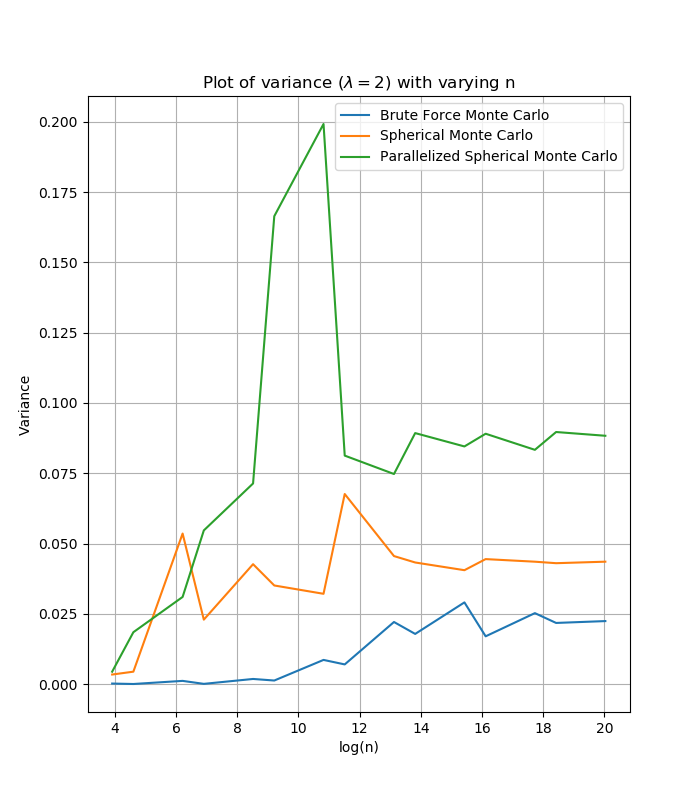
\includegraphics[width = 11cm]{images/variance-montecarlo.png}
    \caption{The plot of variance as a function of the logarithm of integration points $n$ for brute force Monte Carlo, spherical Monte Carlo, and parallelized spherical Monte Carlo. }
    \label{fig:variancemontecarlopng}
  \end{figure}


  \begin{table}[ht]
    \centering
    \caption{Error and execution time for brute force Monte Carlo, spherical Monte Carlo, and parallelized spherical Monte Carlo when testing different compiler optimalization flags with $\lambda = 2$.}
    \vspace{2mm}
    \label{tab:optimalization-montecarlo}
    \begin{tabular}{|c|c|c|c|c|c|c|c|}
        \hline
        Compiler flag & $n$ & BMC error & SMC error & PSMC error & BMC time & SMC time & PSMC time  \\
        \hline \hline
        none & 500000000 & 6.07925e-05 & 2.59234e-05 & 1.66251e-05 & 415.953 & 448.229 & 208.211 \\
        -O & 500000000 & 0.001144 & 3.8324e-05 & 5.9218e-05 & 140.108 & 170.505 & 75.0108 \\
        -O0 & 500000000 & 9.9830e-05 & 1.5527e-05 & 8.7296e-05 & 368.159 & 429.329 & 197.266 \\
        -O1 & 500000000 & 0.0005797 & 2.9770e-05 & 3.3298e-05 & 206.356 & 231.86 & 113.938 \\
        -O2 & 500000000 & 4.7324e-05 & 4.7423e-05 & 2.5998e-05 & 138.492 & 168.688 & 74.8991 \\
        -O3 & 500000000 & 0.001158 & 0.0001025 & 7.5507e-06 & 141.051 & 160.792 & 71.5184 \\
        \hline
    \end{tabular} \\
    \hspace{0pt}\\
  \end{table}
\fi


%--------------- Discussion ---------------------------------------
\vspace{1cm}

\clearpage
\newpage

\section{Discussion} \label{sec:Discussion}




%---------------Conclusion and perspective---------------------------
\vspace{1cm}

\section{Conclusion and perspective} \label{sec:Conclusion}



%--------------Appendix---------------------------------------------
\vspace{1cm}

\section{Appendix} \label{sec:Appendix}



%\clearpage

%----------------References----------------------------------------

\vspace{1cm}

\section{References} \label{sec:References}

\begin{thebibliography}{}

\bibitem{task}
Morten H. Jensen (2019), \href{https://github.com/CompPhysics/ComputationalPhysics/blob/master/doc/Projects/2019/Project3/pdf/Project3.pdf}{Project 3}, Departement of Physics, University of Oslo, Norway

\bibitem{github}
Erik B. Grammeltvedt, Alexandra Jahr Kolstad, Erlend T. North (2019), \href{https://github.com/Erikbgram/Fys3150}{GitHub}, Students of Departement of Physics, University of Oslo, Norway

\bibitem{lecture_slides}
Morten H. Jensen (2015), \href{https://github.com/CompPhysics/ComputationalPhysics/blob/master/doc/Lectures/lectures2015.pdf}{Lecture slides for FYS3150}, Department of Physics, University of Oslo, Norway

\bibitem{laguerre_polynomial}
Weisstein, Eric W. \href{http://mathworld.wolfram.com/LaguerrePolynomial.html}{"Laguerre Polynomial."}, From MathWorld--A Wolfram Web Resource.


\end{thebibliography}


%----------------Slutten av dokumentet---------------------------------------


%\end{multicols}

\end{document}
